% David: FOR MY REVIEW I AM LEAVING COMMENTS LIKE THIS. The idea is that you can tell me if you agree and then we can act on them. I am not leaving comments in stuff that can just be rewritten in a less wordy matter without changing the content

This chapter details the processes and decisions underlying the composition of the model used to answer the research question. Model specification, settings, validation and verification, and experimental setup are established.

\subsection{How is System Dynamics used?}
% David: restructure this: Model has stock, feedback and accumulation, therefore, SD, which is suited for that, is used. Can probably shed a couple words like that

An essential aspect of system dynamics models are accumulations, delays and feedbacks \parencite{sterman_system_2001}. This is suited to the system we wanted to model, and appropriate variables were chosen to represent these features. Infected populations of humans and chickens are modelled as stocks, whilst various transmission routes provide flow variables between them. Feedback loops are modelled as the number of contaminated chicken flocks causes more spread of \textit{Campylobacter} in the environment, and more chickens are infected. Delays are present both in the dynamics of contamination and in implementing policies to slow or suspend transmission.

%1.	Explain basics of SD
 %   a.	Basics of SD
  %  b.	Examples from literature to clarify and justify modelling choices given problem in the field
%2.	Conceptualisation
  %  a.	Depict aggregate model structure
   % b.	Describe dynamic hypothesis

\subsection{Conceptualisation}
\label{s:conceptualisation}
The model focuses on public health and economic impacts associated with \textit{Campylobacter}-contaminated chicken meat. The dynamic hypothesis includes three KPIs that will be examined to answer the research question: 
\begin{itemize}
    \item \textbf{Contaminated Chicken Meat}: part of the infected chicken submodel. This KPI is expected to increase with worsening climate conditions and no interventions.
    % \item Concentration of \textit{Campylobacter} in surface waters: as climate effects continue on their current trends, \textit{Campylobacter} will be able to proliferate more easily and consequently contaminate more poultry meat. This contamination would follow an S-growth curve in the coming years considering both a reinforcing loop of the number of contaminated chicken flocks, causing more spread of 
    % \textit{Campylobacter} in the environment, and in turn the more \textit{Campylobacter} in the environment, the more easily chicken flocks are infected, but also a balancing loop as surface waters will reach a certain carrying capacity. 
    % --> This one is non-existent anymore 
    \item \textbf{Environmental transmissions via disease vectors}: expected to increase with worsening climate conditions that reinforce disease vector prevalence and reinforce transmission routes, and decrease when vectors diminish.
    % the prior KPIs would consequently mean that these would also increase drastically, as most transmission routes are likely to display interaction effects.
    % \item Number of infected people: is expected to increase exponentially as reinforcing loops between farms and environment would greatly increase chance of infection but with a less exponential rate than that of infected flock, as different existing hygiene measures exist to reduce/minimise contamination of meat products.
    \item \textbf{Cost of illness}: is expected to increase with increasing \textit{Campylobacter} infection rates, and decrease (at different rates) with the introduction of different policies.
\end{itemize}
 
\begin{figure}[h]
\centering
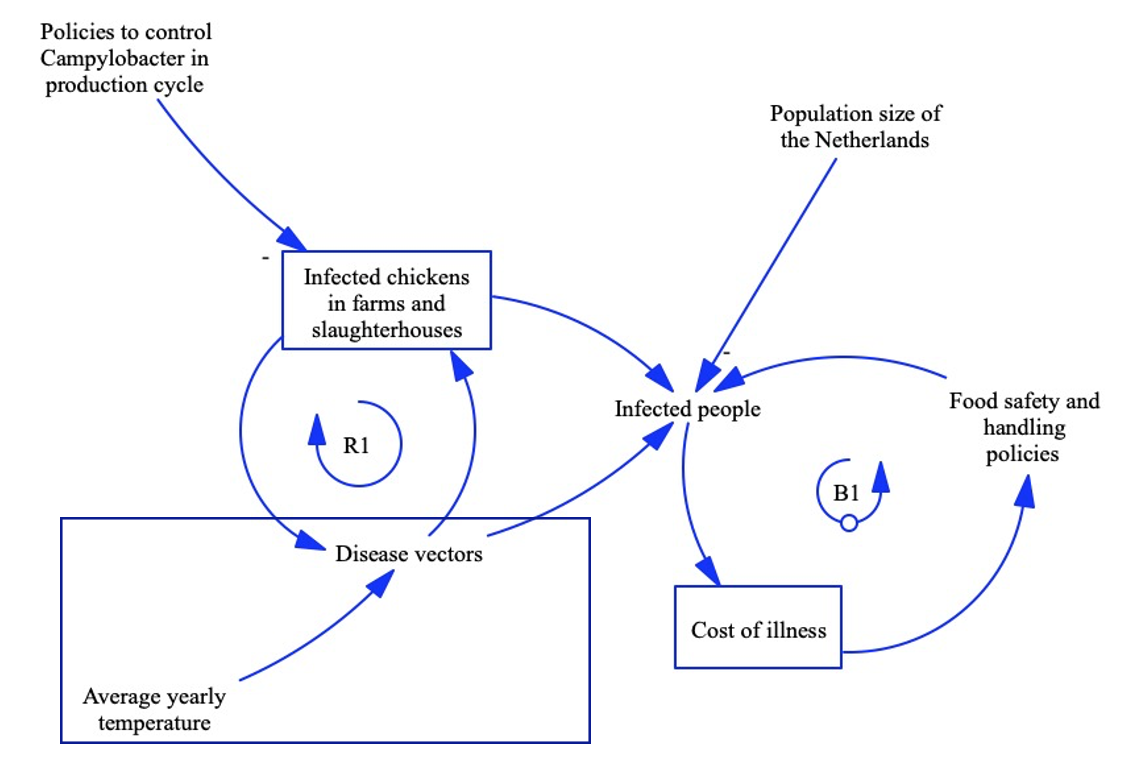
\includegraphics[width=0.65\textwidth]{images/dynamic_hypo2.png}
\caption{The aggregated causal loop diagram for the dynamic hypothesis}
\label{fig:aggregrated_cld}
\end{figure}
 
\subsubsection*{Model Structure}
Conceptualisation of the model structure is shown in Figure \ref{fig:aggregrated_cld}. The model will focus on farms and slaughterhouses collectively, rather than individual types of farms. This aligns better with decision-making regarding the aggregate impacts of policy choices across the entire poultry industry in the Netherlands. This aggregation level excludes most of the internal processes of slaughterhouses and broilers, as these are too detailed for this scope. Furthermore, this model will not be using age cohorts because the public health and cost of illness metrics already incorporate age weightings \parencite{mangen_campylobacteriosis_2007}.  %David: did we introduce the definition of DALYs already before this? Emily: No, I just defined the acronym. We included it in earlier work, but it might have been removed at some stage. DALYs are explained in the model explanation section.
\subsubsection*{Model Boundaries}

This model draws wider boundaries than Rommens' original model \parencite{rommens_infected_2020}. This work focuses on climate, population, and policy effects (both on production and consumption) and the subsequent economic impacts of these factors. Moreover, with the internal components of the farms and slaughterhouses simplified, this allows for more focus on environmental transmission pathways. 

The sub-model of 'Infected Chickens' encompasses the relevant features of Rommens' original model \parencite{rommens_infected_2020}. The following sections detail model structure and behaviour. 

\subsubsection*{Dynamic Hypothesis}

This conceptualisation informed the dynamic hypothesis for behaviour of KPIs, shown in Figure \ref{fig:dynamic_hypothesis}. 

\begin{figure}[h]
\centering
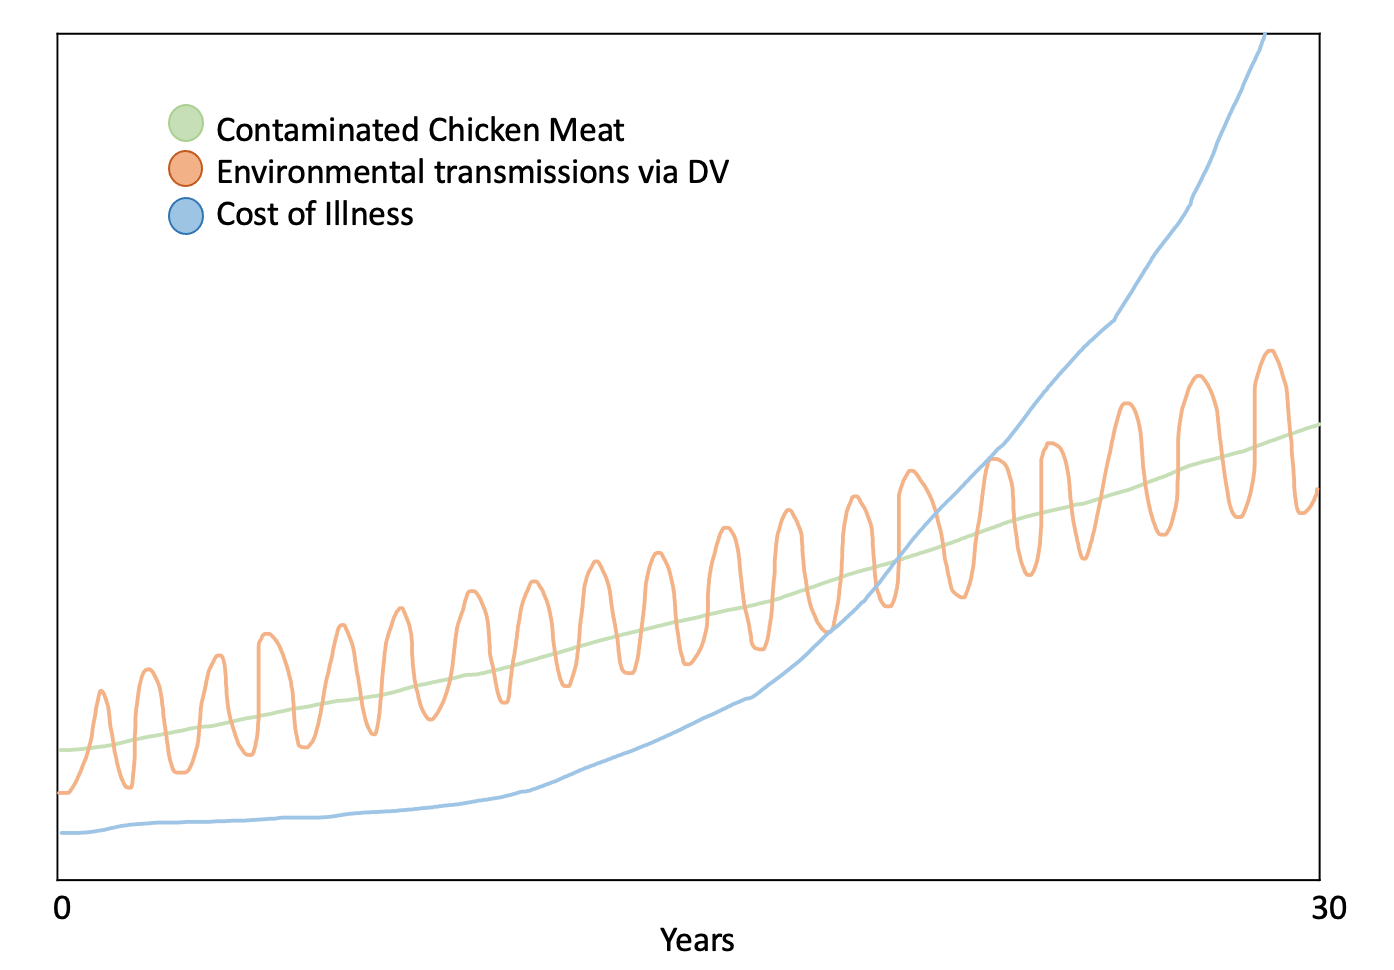
\includegraphics[width=0.50\textwidth]{images/KPI_dynamic_hypo.png}
\caption{Dynamic hypothesis for the KPIs}
\label{fig:dynamic_hypothesis}
\end{figure}

It is hypothesised that the amount of contaminated chicken meat will slowly increase over time because of the reinforcing loop between the chickens and the disease vectors. 
Secondly, it is expected that the effect of disease vectors will follow the temperature as one of the disease vectors (flies) will be more present during the warmer months. Along with climate change, this will slowly increase over time as well. 
Thirdly, the cost of illness will increase exponentially as the chronic cases will accumulate over time. 


\subsection{Model Explanation}
%3.	Explain model (also refer to Appendix A)
 %   a.	Describe sub-models
  %  b.	Explain most important assumptions
   
This analysis contains three main sub-models: environmental transmission, infected chickens and cost of illness. 

%TC:ignore
\iffalse
\begin{itemize}
    \item Environmental %This sub-model focuses on environmental transmission routes and influences for \textit{Campylobacter}, particularly through surface waters and disease vectors (flies and birds other than poultry). According to recent reports by the RIVM, environmental transmission was the second most prevalent cause of \textit{Campylobacter} infections in the Netherlands in 2019. The sub-model also includes levers for climate influences on these transmission pathways.
    \item Infected chickens %This sub-model is based primarily on the work by Rommens. It is a simplified stock-flow model of her original work, designed to replicate key behaviours and interactions.
    \item Cost of illness %This sub-model tracks the impacts and probabilities of \textit{Campylobacter} infections leading to serious illness and fatality, including the relative cost of illness, to reflect economic effects of human \textit{Campylobacter} infections.

\end{itemize}
\fi 
%TC:endignore

\subsubsection*{Environmental}
%IDENTIFY ARCHETYPES

\begin{figure*}[!ht]
	\centering
	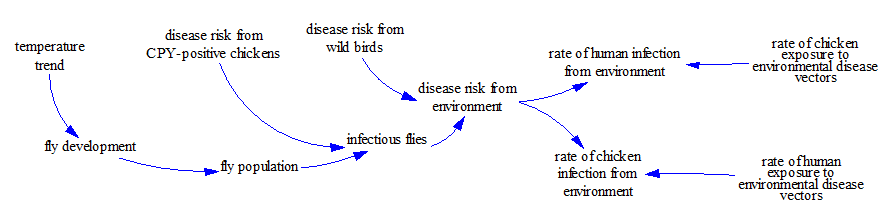
\includegraphics[width=1\textwidth]{images/environmental_submodel2.png}
	\caption{Diagram of the environmental sub-model}
	\label{fig:environmental_submodel}
\end{figure*}


% \textit{Campylobacter} need humid surfaces to live, so surface water is recognised as a key player. Since animal faeces and runoff from agriculture and slaughterhouses enter nearby bodies of water, it is considered a good indicator for the amount of \textit{Campylobacter} present in the environment. Therefore, this has a big role in determining the chance of infection by biological disease vectors mentioned before. This can be seen in Figure~\ref{fig:environmental_submodel}.

The main biological disease vectors have been determined to be flies  \parencite{mughini-gras_quantifying_2016}. Flies are considered to be major spreaders as they actively excrete \textit{Campylobacter} on surfaces and human food \parencite{french_molecular_2009, hald_influxed_2008, berndtson_campylobacter_1996}. We use the common house fly as the model organism to represent the effects of disease vectors \parencite{hald_influxed_2008}. \cite{skovgard_retention_2011} suggests that flies are mainly short distance carriers of \textit{Campylobacter}. Therefore, the risk of transmission by flies particularly high when the populations are greatest, which is during summer \parencite{royden_role_2016}. \cite{hald_use_2007} showed that preventing flies from entering houses in the summer of 2006 caused a significant drop in the prevalence of \textit{Campylobacter} at farms. 
Climate change will cause the number of flies in the Netherlands to increase in both summer and winter \parencite{goulson_predicting_2005}. Rainfall is not a driving factor in the size of the fly population \parencite{goulson_predicting_2005}, and so was excluded from the model as an environmental factor.

%Climate change is also linked to different precipitation patterns in the Netherlands. An increase in precipitation will result in increase of the Dutch sewer systems being overwhelmed and dumping the overflow in the environment, and will also result in an increase of contaminated runoff from agriculture and slaughterhouses \parencite{kwaad_summer_1991}.

An increase in Dutch population size is not expected to increase the fly biomass in the Netherlands \parencite{guenat_effects_2019}. Even though an increase in the population leads to more organic waste \parencite{garcia-garcia_framework_2015}, which does have the potential to increase the total number of flies \parencite{imai_population_1984, rozendaal_houseflies_1997}, this effect is possibly counterbalanced by the loss of natural habitat.

%Effect of climate change on runoff of Campylobacter and Cryptosporidium from land to surface water  This study shows that for the evaluated scenarios, climate change has little impact on concentrations of Campylobacter and Cryptosporidium transported from land to the surface waters.

% Seasonal effect on probability of infection through surface water?

\subsubsection*{Infected chickens}
Figure \ref{fig:transmission_submodel} shows the conceptual dynamics of transmission and contamination in farms, broilers and slaughterhouses \parencite{rommens_infected_2020}. Healthy chickens become infected with \textit{Campylobacter} due to environmental disease vectors \parencite{royden_role_2016}, which themselves become infected from chicken \parencite{skovgard_retention_2011}. These infected chickens then become contaminated chicken meat when slaughtered. They can also cause cross-contamination, making the meat of healthy chicken also potentially contaminated when it enters into contact with the bacteria \parencite{berndtson_campylobacter_1996}. Consumption of contaminated meat may then cause human infection \parencite{wilson_tracing_2008}.

This submodel behaves like the "success to the successful" archetype \parencite{pruyt_triple_2013}, where the feedback loops around the rate of chicken infection imply that when there are fewer infections, it is prone to stay that way. However, when infections rise, it is difficult to limit their growth. The implications for our model is that a slight push in the direction of infections can have significant implications.

\begin{figure}[h!]
\centering
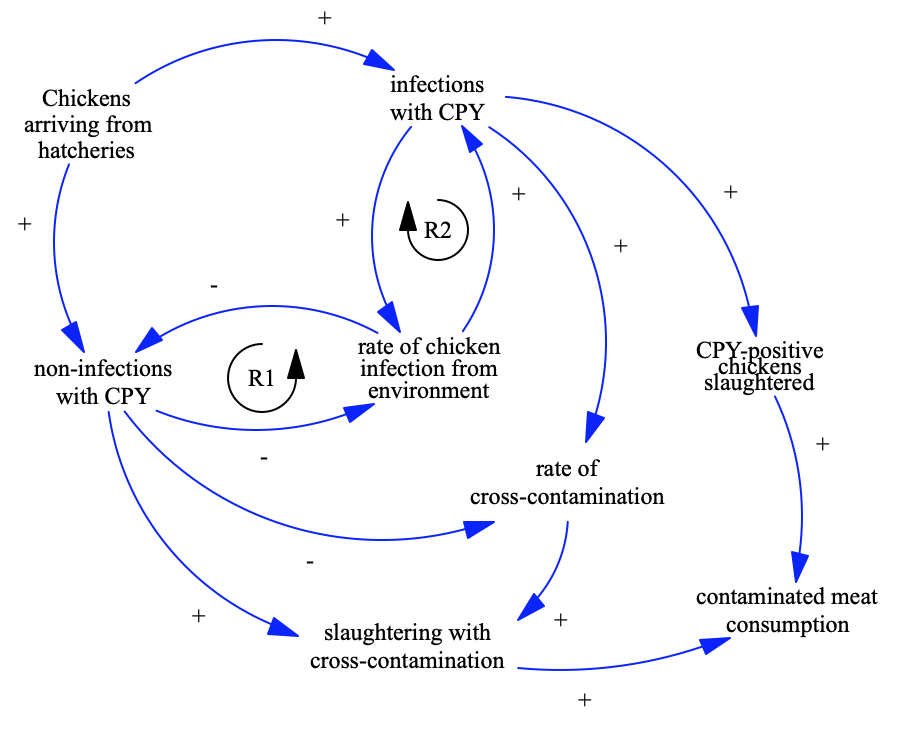
\includegraphics[width=0.50\textwidth]{images/Transmission submodel.png}
\caption{Conceptual causal loop diagram for chicken infection and contamination}
\label{fig:transmission_submodel}
\end{figure}

Other internal variables in this model included probabilities of infection, which are determined by environmental factors such as propagation of disease vectors, with the exact values for these rates detailed in Appendix~\ref{ch:model_documentation}.


\subsubsection*{Cost of illness}

The cost of illness associated with \textit{Campylobacter} infections is modelled and calculated based primarily on a 2007 study by Mangen \parencite{mangen_campylobacteriosis_2007}. The Infected Persons stock is split off into symptomatic and asymptomatic infections. Symptomatic infections are assumed to all develop acute gastroenteritis, with a proportion of all cases recovering or subsequently developing chronic illnesses. Each of these outcomes contribute to public health metrics of Disability Adjusted Life Years (DALYs) for these infections and the Cost of Illness for all \textit{Campylobacter} infections. 

\begin{figure}[h]
\centering
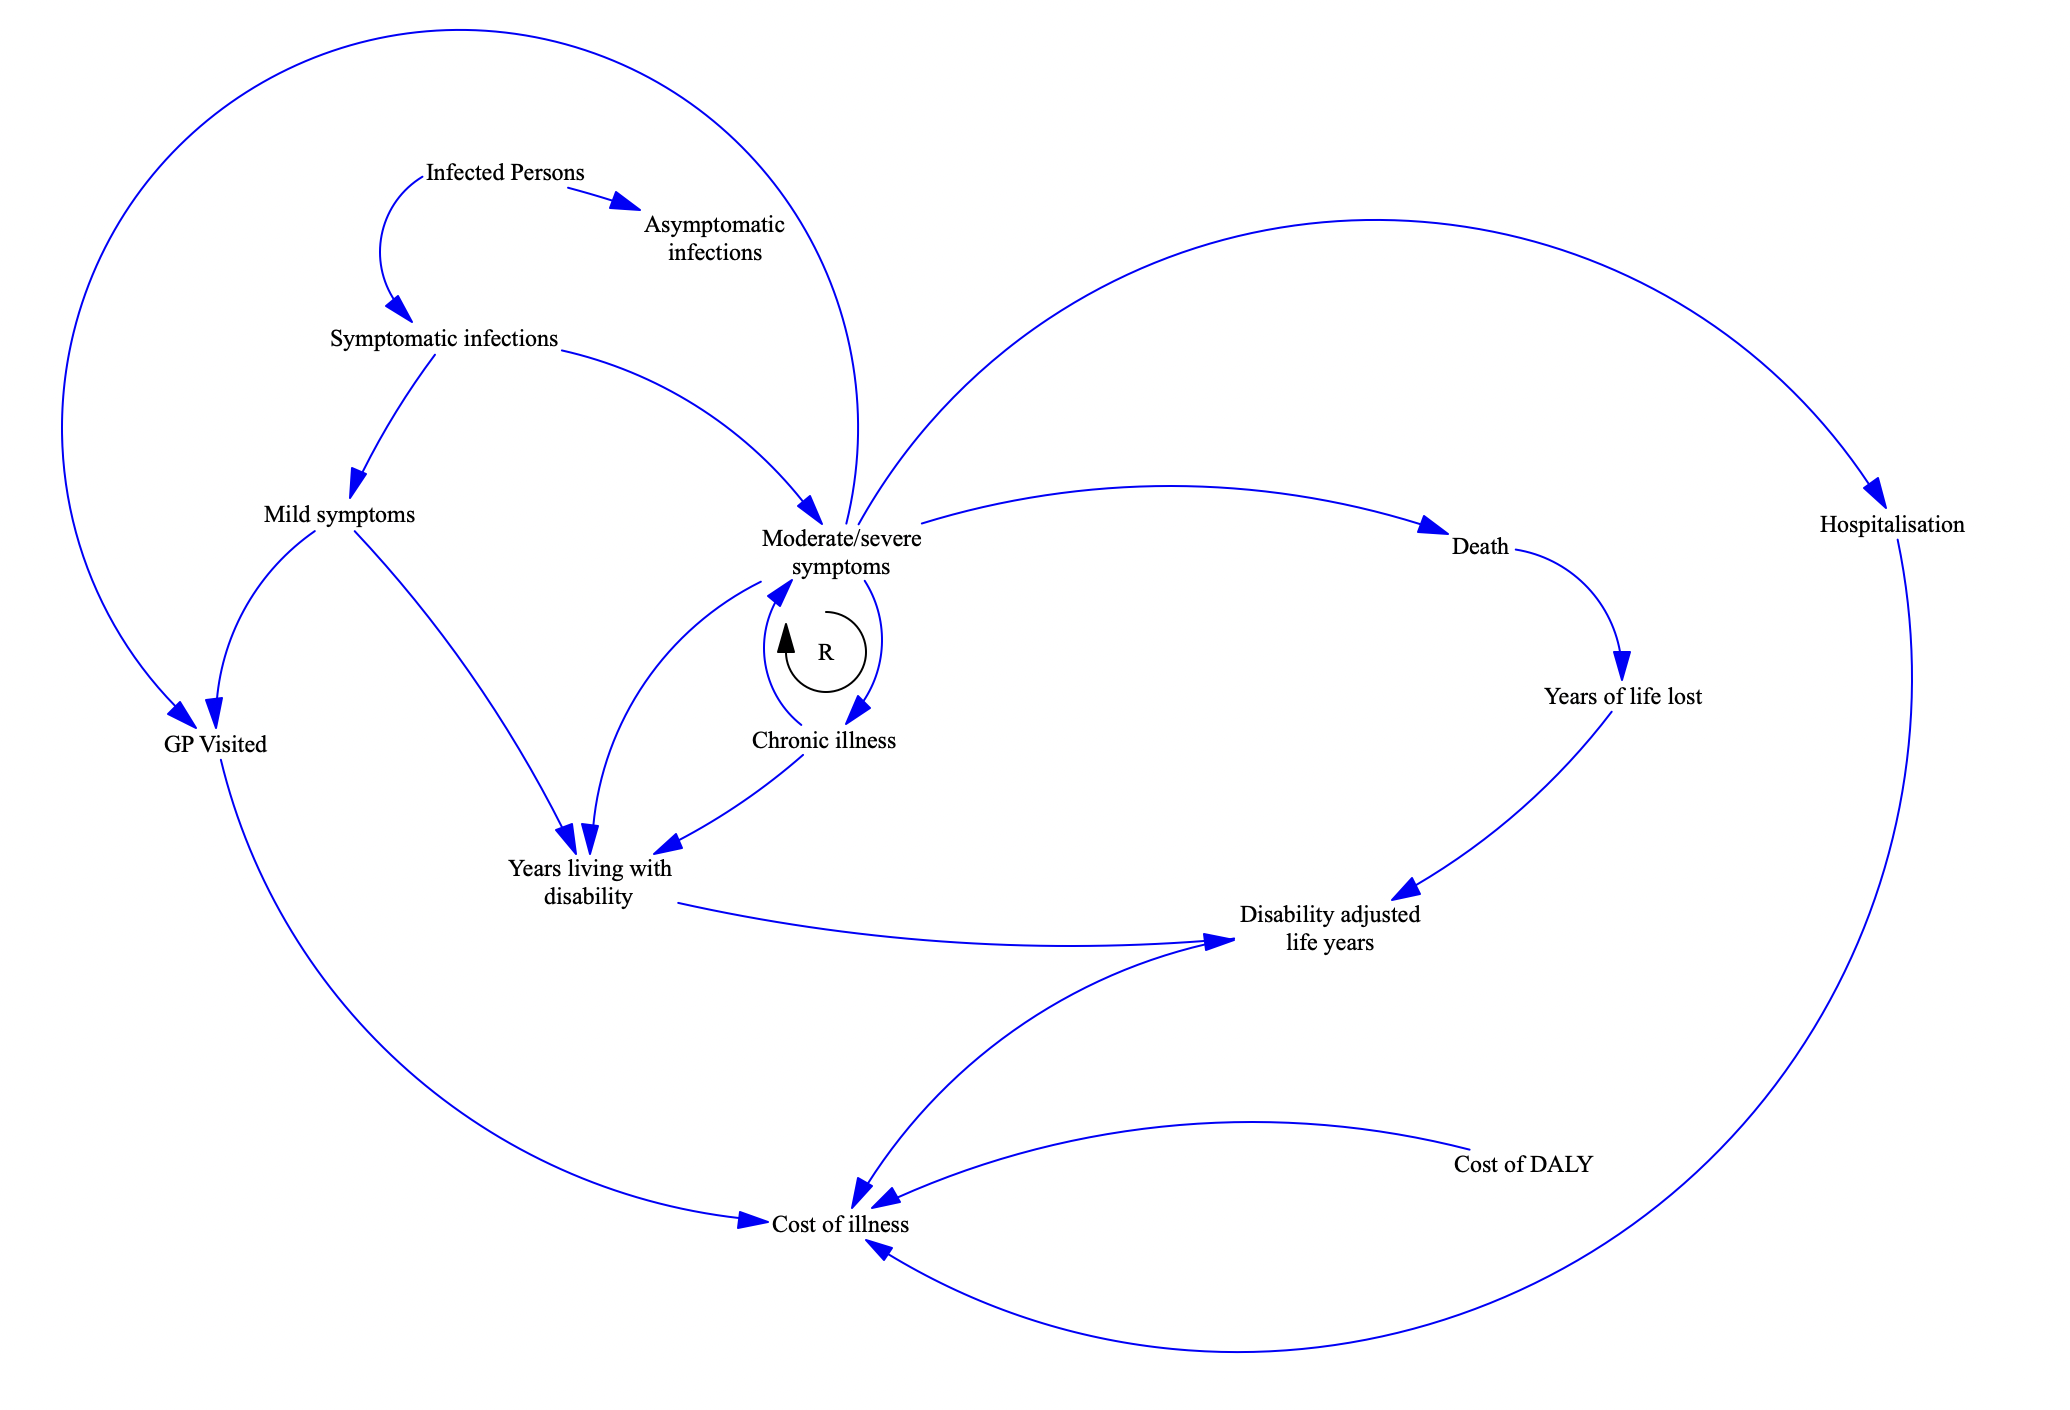
\includegraphics[width=0.75\textwidth]{images/COI_submodel.png}
\caption{The conceptual Cost of Illness sub-model}
\end{figure}

The causal structure adopted for this sub-model focuses on connecting variables based on available scientific data. Due to the underlying complexity of DALYs and Cost of Illness metrics \parencite{jo_cost--illness_2014}, we take a top-down approach to applying these variables. As such, variables have been used for some elements in place of stocks (e.g. DALYs and Cost of Illness). This simplistic approach is considered appropriate as we are not concerned with the details of transmission and recovery, but only with the ultimate KPI 'Cost of Illness'. 

\subsection{Key Assumptions}
\label{s:assumptions}
%What were the key assumptions made in developing the model?
    %Take from validation spreadsheet
    %Include simplifications of real-world circumstances (e.g. acute campy coming before chronic conditions)
The main assumptions made in modelling these causal structures are:
\begin{itemize}
    \item All chicken meat consumed in the Netherlands is produced in the Netherlands and the population of the Netherlands cannot eat more than is produced in the Netherlands.
    \item All infected meat becomes contaminated meat when slaughtering.
    \item Cross-contamination in the slaughtering process depends on the proportion of total infected chickens present at the moment of slaughtering. %This is based on the amount of \textit{Campylobacter} negative chicken, which represents the amount of negative chicken being slaughtered, not merely existing. % David: probs enough to leave only the first sentence
    \item The development of chronic disease is assumed to always occur subsequent to a case of acute gastroenteritis (in reality, some cases will develop chronic disease without first developing gastroenteritis, following a \textit{Campylobacter} infection
    \item There is no recovered population, meaning that infected people are able to be reinfected and do not become immune.
\end{itemize}

% Multiple assumptions on the values of individual parameters have been made, due to the absence of adequate literature. Where this is the case, the assumption has been noted in \textcolor{red}{table x in appendix y}. % David: probs unnecessary

\subsection{Model Specification}
%What are the main mechanisms/variables/parameters/equations in our model?
The main mechanisms employed in each part of the model are as follows:
\begin{itemize}
    \item Environmental transmission: this part of the model replicates empirical models of insect development cycles, and translates this to prevalence of environmental transmission of \textit{Campylobacter} by disease vectors, therefore providing a path of infection for chicken and humans.
    \item Chicken infections: the chicken infections part of the model describes the mechanisms by which environmental infections enter the food supply for human consumption, creating the foodborne infection mechanism.
    \item Cost of Illness: captures the annual consequences of foodborne and environmental \textit{Campylobacter infections} on humans. %the the cost of illness model relies on accumulation over time, while using a pulse-train mechanism to 'empty' the annual occurrence of acute illness.
    
\end{itemize} % David: isn't this the same as talking about the submodels? I say remove, if anything we can briefly say how those models interact with one another. Emily - this is the section I was asking about this morning. Really not sure what we are expected to include here that isn't covered in the model documentation.

A complete list of variables and parameters used in the model are detailed in Appendix \ref{ch:model_documentation}

\subsubsection{Modelling software used}
The system was modelled using VenSim PLE software developed by Ventana Systems Inc.
%Model Settings
    %Why was the integration method chosen?
    
\subsubsection{Integration method}
Euler was considered an adequate integration method for this model as it is suitable for integrating over non-linear and discontinuous functions (such as the pulse trains used to drain some stocks), and it is a simple a direct method of integration. However, it does present some limitations in computational inefficiencies.

\subsubsection{Time step}
    %Why was the time step chosen?
The time step must be small enough such that the derivative of the model is constant between two points close in time. A Time step of 0.0625 was selected, as behaviour of the model was consistent with that of lower time steps (see Figure \ref{fig:cpy cases with time step}).

\begin{figure}[h!]
\centering
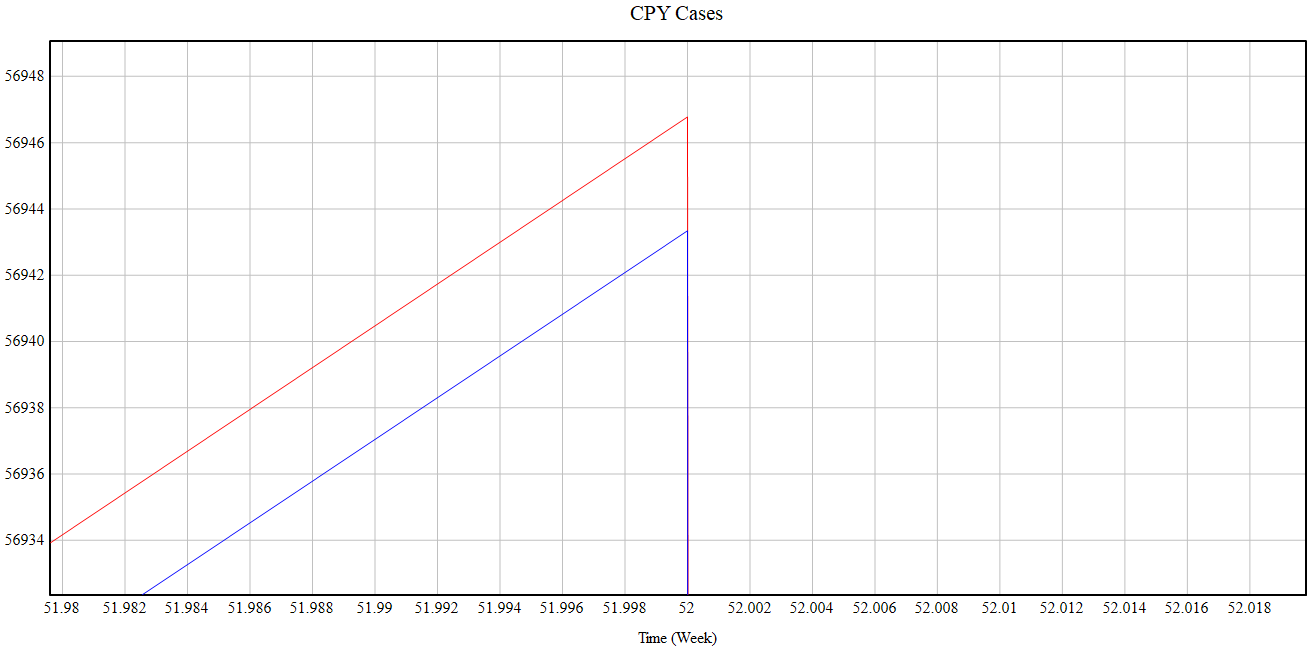
\includegraphics[width=0.65\textwidth]{images/timestep.PNG}
\caption{Peak CPY Cases with time steps 0.0625 and 0.03125}
\label{fig:cpy cases with time step}
\end{figure}

Results of this model are presented starting at the 53rd week (1 year and 1 week through the simulation). This is to allow for the model behaviour to be stabilise, since all stocks are given initial values of zero. This also allows for behaviour to be reported starting in the year 2021.

\subsubsection{Time period}
    %Why was the time period chosen
The time period of 30 years (1560 weeks) was chosen to be able to show the effects of incremental changes in climate variability, however, since the impact of worsening climate conditions is tightly linked to seasonality, the time unit was weeks. % for the purpose of maintaining a small enough time step unit such that the transmission within chicken farms is realistic,

\subsection{Model Verification and Validation}
%4.	Validation
 %   a.	Use various tests to argue why model is fit for purpose
In this subsection the model will be undergo verification and validation. Verification will be done through a comparison with the conceptualisation of the model, as well as a unit and a time step verification. 

\subsubsection{Verification}
\label{s:verification}

% From meeting with Jill:
%Verification requires three steps:
    %Check that the causal diagrams match the stock-flow diagrams, and add one line saying "this was checked'
    
To verify the conceptualisation, the causal diagram construed in chapter \ref{s:conceptualisation} was compared with the model built. There have been some addenda to the model, but the functions still match.  
    %Check that the units are consistent with the real world and add one line saying 'units were checked for material consistency'. -- DONE
    
Units were checked to ensure consistency with real-world equivalents. The only noteworthy unit is that of the flow \textit{Symptomatic infections}. The model's time unit is set to \textit{week}, to facilitate seasonal temperature throughout the year. As DALY and COI are reported per year, a PULSE TRAIN function is modelled between stocks \textit{CPY Cases} and \textit{Acute GE Cases} to convert time units. This accumulates all \textit{Campylobacteriosis} cases over 52 weeks before transferring them to the cost of illness submodel. This 'transforms' the unit into years for the COI submodel. The units of the PULSE train remain in weeks when the time unit should be thought of as year, as happens after. 
    %Confirm that you've used the appropriate numerical technique/time step and add one line saying, 'behaviour of the model for the chosen time step and half that time step is consistent, this indicates that the appropriate time step and integration method has been used'
    
The time step verification was performed by running the model at several different time steps. The time step 0.0625 is chosen so the integration method (Euler) is valid. When halving the time step, we found that model returned similar model behaviour, 

%with the exception of one flow, the \textit{symptomatic infections}. This is because this flow uses a PULSE TRAIN, as described above and this pulse train depends on the time step. Because of this, when the time step is halved, the PULSE TRAIN becomes far bigger. However, this has no effect on the stock it goes into, the number of acute cases. 
% David: excepting the specific explanation of the pulse train, everything here has already been tackled

%Concerning the time step, we found that the \textit{symptomatic infections} flow changed depending on the used time step. This is because this flow uses a PULSE TRAIN, as described above. Because of this, when the time step is halved, the PULSE TRAIN becomes far bigger. However, the result of this integration is the same, so it has no different effect on the stock it goes into.

\subsubsection{Validation}    

%Validation requires three steps:
    %Show how the data matches or does not match historical data (explain why)

Several tests were performed to ascertain whether the model was fit for purpose \parencite{forrester_tests_1980}. The complete Validation can be read in Appendix~\ref{ch:validation}.

The appendix also elaborates on the model boundary. The model boundary determines the kind of policies that can be tested, and also vice versa, the policies we were interested in shaped the model boundary. We included the pathways we deemed interesting for our research question, and the tests we have performed are only concerned with these pathways.

To find the boundaries withing which the model works, we tested extreme conditions. The first and most obvious boundary is regarding time, as the \textit{final time} of the model cannot be higher than 30 years, since information such as temperature increase due to climate change and population projections are only defined until that date. Other extreme conditions tested can be found in table \ref{tab:extreme_values_results}.

%TC:ignore
\begin{longtable}[c]{m{8em} m{2em} m{2em} m{22em}}
\caption{Variable values used for extreme conditions testing and test results.}
\label{tab:extreme_values_results}\\
\hline
Variable & Extreme low & Extreme high & Result \\
\hline
\endfirsthead
%
\endhead

\textit{Temperature increase by 2050}   &   -1          &   25              &   Model breaks under extreme high condition, but behaves as expected under extreme low. \hline \\
\textit{Initial fly population}         &   0           &   1               &   Model breaks under extreme high condition, but the data from the first year has already been deemed inaccurate, thus, the model could still be used. The model behaves as expected for extreme low.   \hline \\
\textit{Chicken arriving from hatcheries} & Halved      &   Doubled         &   Model breaks under extreme high condition, but behaves as expected under extreme low. \hline \\
\textit{Infections per kg of meat consumed} &   Halved  &   20x             &   Model breaks under extreme high condition, but behaves as expected under extreme low. \hline \\
\textit{Base infectious flies}          &   0           &   0.8             &   Model breaks under extreme high condition, but behaves as expected under extreme low. \hline \\
\textit{Base chicken exposure rate}     &   0           &   0.8             &   Model breaks under extreme high condition, but behaves as expected under extreme low. \hline \\
\textit{CPY reproduction in chickens}   &   0           &   4               &   Model breaks under extreme high condition, but behaves as expected under extreme low. \\ \hline
\end{longtable}
%TC:endignore

Next we conducted multiple sensitivity analyses. We found that the system is fairly reliable when in the univariate tests. The results of the multivariate sensitivity analysis showed that there is quite some numeric sensitivity. This is mainly due to people changing their consumer behaviour, and meat piling up as a result.

Finally we compared our model to real world data, and made the following observations:
\begin{itemize}
    \item The number of people with campylobacteriosis is slightly higher in the model than in the estimates, but the difference is within an acceptable range.
    \item Most of the cases of campylobacteriosis originate from the environment and not from poultry consumption, conform to literature.
    \item The proportion of infected chickens in the base model corresponds to the expected proportion in the real world.
    \item The model calculates more DALYs than the literature, which may be an indication that doctors are sometimes unable to trace the diagnosis back to \textit{Campylobacter}.
    \item The Cost of Illness is lower than the literature. This is probably due to the fact that we only look at acute cases and three chronic diseases. The values used are also indexed to prices from the year 2000. It's recommended that model users apply an institutionally appropriate inflation figure.
\end{itemize}

%TC:ignore
\iffalse
\textbf{Extra}\\
\textcite{vlaanderen_staat_2019} and curperus also show the actual human infections confirmed by laboratoria from 2006-2018, and the numbers for the Netherlands. I assumed these were uninteresting, since we also care about untested individuals

The use of antacids may increase one's chances of getting Campylobacteriosis. This is structural uncertainty we could include.

\textcite{vlaanderen_staat_2019} shows that \textit{Campylobacter} is becoming resistant against antibiotics: also uncertainty.


I suppose the factor wild birds play can also be considered uncertain. There are still a lot of gaps in the literature regarding disease transmission amongst birds and from birds to other animal taxa.
\fi
%TC:endignore





%The extreme high value of \textit{temperature increase} evidences a problem in the model, as fly reproduction is unreasonably high since extreme temperatures are likely to create a harsher environment for them as well. For the extreme high values of \textit{initial fly population}, \textit{CPY reproduction in chickens}, and \textit{base chicken exposure rate} In the model reports a proportion of contaminated meat that is greater than the total amount of meat, which should not be possible. A similar thing happens with \textit{base infections flies}, which can cause more infectious flies than there are total flies. When \textit{chicken arriving from hatcheries} are decreased (and thus made lower than the demand), the model can handle the situation because it does not allow for consumption of more chicken that are available, but when instead it is raised, the excess supply is never dumped, creating an issue of accumulating meat indefinitely which is not realistic. Lastly, when \textit{infections per kg of meat} consumed are raised 20 times its original value, it can bring issues of too many people being infected, since our model does not account for immunity of population, all population is indefinitely susceptible which becomes a problem when infection numbers are very big.% David: I feel like this could be restructured, and some of it might be fully sent to the appendix, but I'm not sure how to tackle it. Maybe add an additional column in the table above?
% Screw it, I'm modding the table

Visualisations for these situations can be found in Appendix \ref{s:extreme_conditions}.
    
    %Generate the mode of behaviour/dynamic hypothesis - does it match, why or why not?
% Refer to Section \ref{s:b_base} where the behaviour of the base model without policies is examined. In this section, the differences and similarities between the model and the dynamic hypothesis are discussed.
The output of the model matches the dynamic hypothesis, with some minor differences. Visualisations and commentary on model performance relative to the dynamic hypothesis is given in Section \ref{s:baserun}
    
\subsection{Experimental setup}
%5.	Experimental setup
 %   a.	Introduce main uncertainties (potentially with table)
  %  b.	Explain scenario and policy logic
  
        %Parametric experiments - change parameters and observe behaviour (do multivariate for all, and univariate for one or two key variables)
        %Structural experiments - change a structure (e.g. add feedback) and observe behaviour 
   % c.	Number of runs, numerical integration method & time step, versions, etc.: all justified
To answer our research question, experiments were set up around the three components in the research question: climate, population and public health. 

We identified a number of uncertainties in the model that are summarised in Table \ref{tab:uncertainties}. Parametric uncertainties will be used to perform sensitivity analysis in the model, whereas most structural uncertainties will be explored to define possible policy interventions.
%TC:ignore
\begin{longtable}[]{l|l|l}
\caption{Summary of uncertainties in the system}
\label{tab:uncertainties} \\
\hline
\textbf{Type}                  & \textbf{Parametric}                                                                        & \textbf{Structural}                                                                                         \\ \hline
\multirow{2}{*}{Population}    & \multirow{2}{*}{Population projections}                                                    & Chicken consumption behaviour                                                                                \\
                               &                                                                                            & Food safety in handling                                                                                     \\ \hline
\multirow{2}{*}{Climate}       & \multirow{2}{*}{Temperature projections}                                                   & Climate effects of temperature seasonality                                                                  \\
                               &                                                                                            & \begin{tabular}[c]{@{}l@{}}Pest control measures to limit spread of \\ disease vectors\end{tabular}         \\ \hline
\multirow{2}{*}{Public health} & Cost of illness                                                                            & \begin{tabular}[c]{@{}l@{}}Slaughterhouse hygiene regulations \\ to reduce cross-contamination\end{tabular} \\ 
                               & \begin{tabular}[c]{@{}l@{}}Proportion of people developing \\ chronic illness\end{tabular} & Limit exposure to flies                                                                                     \\ \hline
\end{longtable}
%TC:endignore

The structural and parametric uncertainties resulted in five policies that will be tested. These policies were designed based on reality and are capable of providing a view of the policies' cost effectiveness and robustness. 

The parametric uncertainties were used to devise a sensitivity analysis and scenario tests for robustness of the policy. The parameters are the projection of the Dutch population, the temperature increase in the coming 30 years and the cost of illness. 

\subsubsection{Policies tested}

The policies tested on the model were implemented as described in Table \ref{tab:policies}.

%TC:ignore
\begin{table}[h!]
\centering
\caption{Policies tested and their parameterisation}
\begin{tabular}{ l  p{3.8cm}  p{3.8cm}}
\hline
Policy Name &
   Description &
  Parameterisation \\ \hline
Exposure Control &
  Public campaigns to control human exposure to infected flies &
  Reduce human exposure to flies by 20\% with delay of one week \\
Pest Control &
  Extermination of flies in infection prone areas &
  Reduce 'infectious flies variable' by 20\%, triggered by temperature above 20 degrees \\
Consumption Behaviour &
  Public campaign encouraging population to reduce chicken meat consumption when case numbers are high &
  Reduce 'consumption rate per person' by 0.05 kg/week/person \\
Food Safety and Handling &
  Public campaign encouraging improved household food hygiene &
  Reduce infections per kg of meat consumed by 20\% \\
Safe Slaughtering &
  Require slaughterhouses to implement more hygiene measures &
  Reduce rate of cross contamination by 20\% \\ \hline
\end{tabular}
\label{tab:policies}
\end{table}
%TC:endignore

%TC:ignore
\iffalse
\begin{itemize}
    \item Public campaigns to control human exposure to infected flies: when disease vectors (flies) are more prevalent, the government requires the population to keep organic waste properly closed and use fly nets \parencite{hald_use_2007}.
    \item Pest control measures: when average temperatures are above 20 degrees Celsius, the government can initiate fly extermination campaigns to limit the spread of diseases.
    \item Improve sanitation of slaughterhouse process and equipment: requirement for slaughterhouse equipment to be cleaned using water that is frequently changed to prevent cross-contamination. This can also be enhanced by the use of UV radiation to aid in the decontamination process without altering the sensory quality of the meat \parencite{isohanni_use_2009}.
    \item Food safety and handling: Policy connecting cost of illness to proportion of contaminated chicken
    \item Behavioural link from DALYs to either infections per kg consumed OR kg of chicken meat consumed. There is a structural uncertainty related to how consumer behaviour might change. Will individuals reduce their chicken consumption or will they be more careful in food handling?
\end{itemize}
\fi
%TC:endignore

%FOR WHOMEVER IT MAY CONCERN: at the moment there is no duplicate of the following subsubsection in policies.tex.
\subsubsection*{Note on policy implementation}
Policies were implemented using switches, connecting directly to the variable it is meant to address. This is not realistic as policies will exhibit side effects. To more accurately integrate policies into the system,  a group modelling approach is recommended, including relevant stakeholders such as farmers, policy experts, and public health practitioners \parencite{vennix_group_1999}. %David: wouldn't this be more of a limitation and recommendation?

\subsubsection{Scenarios tested}
Policies were tested for robustness under different population, temperature change, seasonality and public health scenarios, as shown in Appendix \ref{ch: detexp}.


Specific details on the policies and on their implementations within the model can be read in Appendix~\ref{ch:det_policies}.